\documentclass[a4paper, 11pt]{article}
\usepackage{comment} % enables the use of multi-line comments (\ifx \fi) 
\usepackage{lipsum} %This package just generates Lorem Ipsum filler text. 
\usepackage{fullpage} % changes the margin
\usepackage{graphicx}
\usepackage[colorlinks]{hyperref}
\usepackage[nameinlink,noabbrev]{cleveref}
\usepackage{color}
\graphicspath{ {./images/} }

\begin{document}

\noindent
\large\textbf{Tema de cas\u{a}} \hfill \textbf{Programarea Aplica\c{t}iilor \^{i}n Timp Real} 
\begin{flushright} Sem. 2, 2021-2022 \end{flushright} 
\hfill \break
\normalsize Echipa: APOSTU \c{S} Raluca, \space\space\space\space PLESCA Natalia, \space\space\space\space\space CONTIU Alexandru\\
\normalsize e-mail: \space raluca.marian54@yahoo.com, plescanatalia2000@gmail.com, contiu.marian@gmail.com\\
\\
\large\textbf{\textcolor{blue}{INTERSEC\c{T}IE SEMAFORIZAT\u{A}}}

\section{Introducere - prezentarea problemei}
Problema pe care echipa noastr\u{a} a abordat-o este aceea a unei intersec\c{t}ii semaforizate. Procesele vor fi reprezentate de st\u{a}rile unui semafor \c{s}i direc\c{t}iile de mers ale \c{s}oferilor.

\subsection{Exemplu: Pas 1. Definire problem\u{a}}
Se va implementa o aplica\c{t}ie format\u{a} din 4 taskuri:

\begin{itemize}
\item Task 1 (func\c{t}ia PerecheA) - semafoarele pentru vehicule (V2, V3) devin ro\c{s}ii,  \^{i}n timp ce semafoarele pentru vehicule (V0, V1) \c{s}i cele pentru pietoni (P2, P3)  \^{i}\c{s}i schimb\u{a} starea din ro\c{s}u  \^{i}n verde;
\item Task 2 (func\c{t}ia Tranzi\c{t}ieAB) - pentru a avertiza \c{s}oferii de pe \c{s}oseaua vertical\u{a} cu privire la schimbarea culorii semafoarelor, semafoarele pentru vehicule (V0, V1)  \^{i}\c{s}i schimb\u{a} culoarea  \^{i}n galben, semafoarele pentru pietoni (P2, P3) se fac ro\c{s}ii, iar celelalte semafoare  \^{i}\c{s}i p\u{a}streaz\u{a} starea;
\item Task 3 (func\c{t}ia PerecheB) - semafoarele pentru vehicule (V0, V1) devin ro\c{s}ii,  \^{i}n timp ce semafoarele pentru vehicule (V2, V3) \c{s}i cele pentru pietoni (P0, P1)  \^{i}\c{s}i schimb\u{a} starea din ro\c{s}u  \^{i}n verde;
\item Task 4 (func\c{t}ia Tranzi\c{t}ieBA) - pentru a avertiza \c{s}oferii de pe \c{s}oseaua orizontal\u{a} cu privire la schimbarea culorii semafoarelor, semafoarele pentru vehicule (V2, V3)  \^{i}\c{s}i schimb\u{a} culoarea  \^{i}n galben, semafoarele pentru pietoni (P0, P1) se fac ro\c{s}ii, iar celelalte semafoare  \^{i}\c{s}i p\u{a}streaz\u{a} starea.
\end{itemize}
Condi\c{t}iile de schimbare a culorii semaforului sunt urm\u{a}toarele:


\begin{itemize}
\item Condi\c{t}ia 1 - semafoarele de pe \c{s}oseaua vertical\u{a} \c{s}i cele de pe \c{s}oseaua orizontal\u{a} nu pot indica culoarea verde sau galben\u{a}  \^{i}n acela\c{s}i timp;
\item Condi\c{t}ia 2 - semafoarele pentru pietoni de pe o \c{s}osea nu pot fi verzi at\^{a}ta timp c\^{a}t semafoarele pentru vehicule de pe acea \c{s}osea sunt verzi sau galbene;
\item Condi\c{t}ia 3 - tranzi\c{t}iile (culoarea galben \u{a}) sunt condi\c{t}ionate de un interval de 5 secunde, iar st\u{a}rile (culoarea ro\c{s}ie sau verde) sunt condi\c{t}ionate de un interval de 10 secunde.
\end{itemize}


\section{Analiza problemei}

\subsection{Exemplu: Pas 2. Analiza cerin\c{t}elor} 
Secven\c{t}ele posibile sunt ilustrate \^{i}n \autoref{fig:tasks} (aceast\u{a} reprezentare este metoda de afi\c{s}are din terminal). 
\begin{figure}
\centering
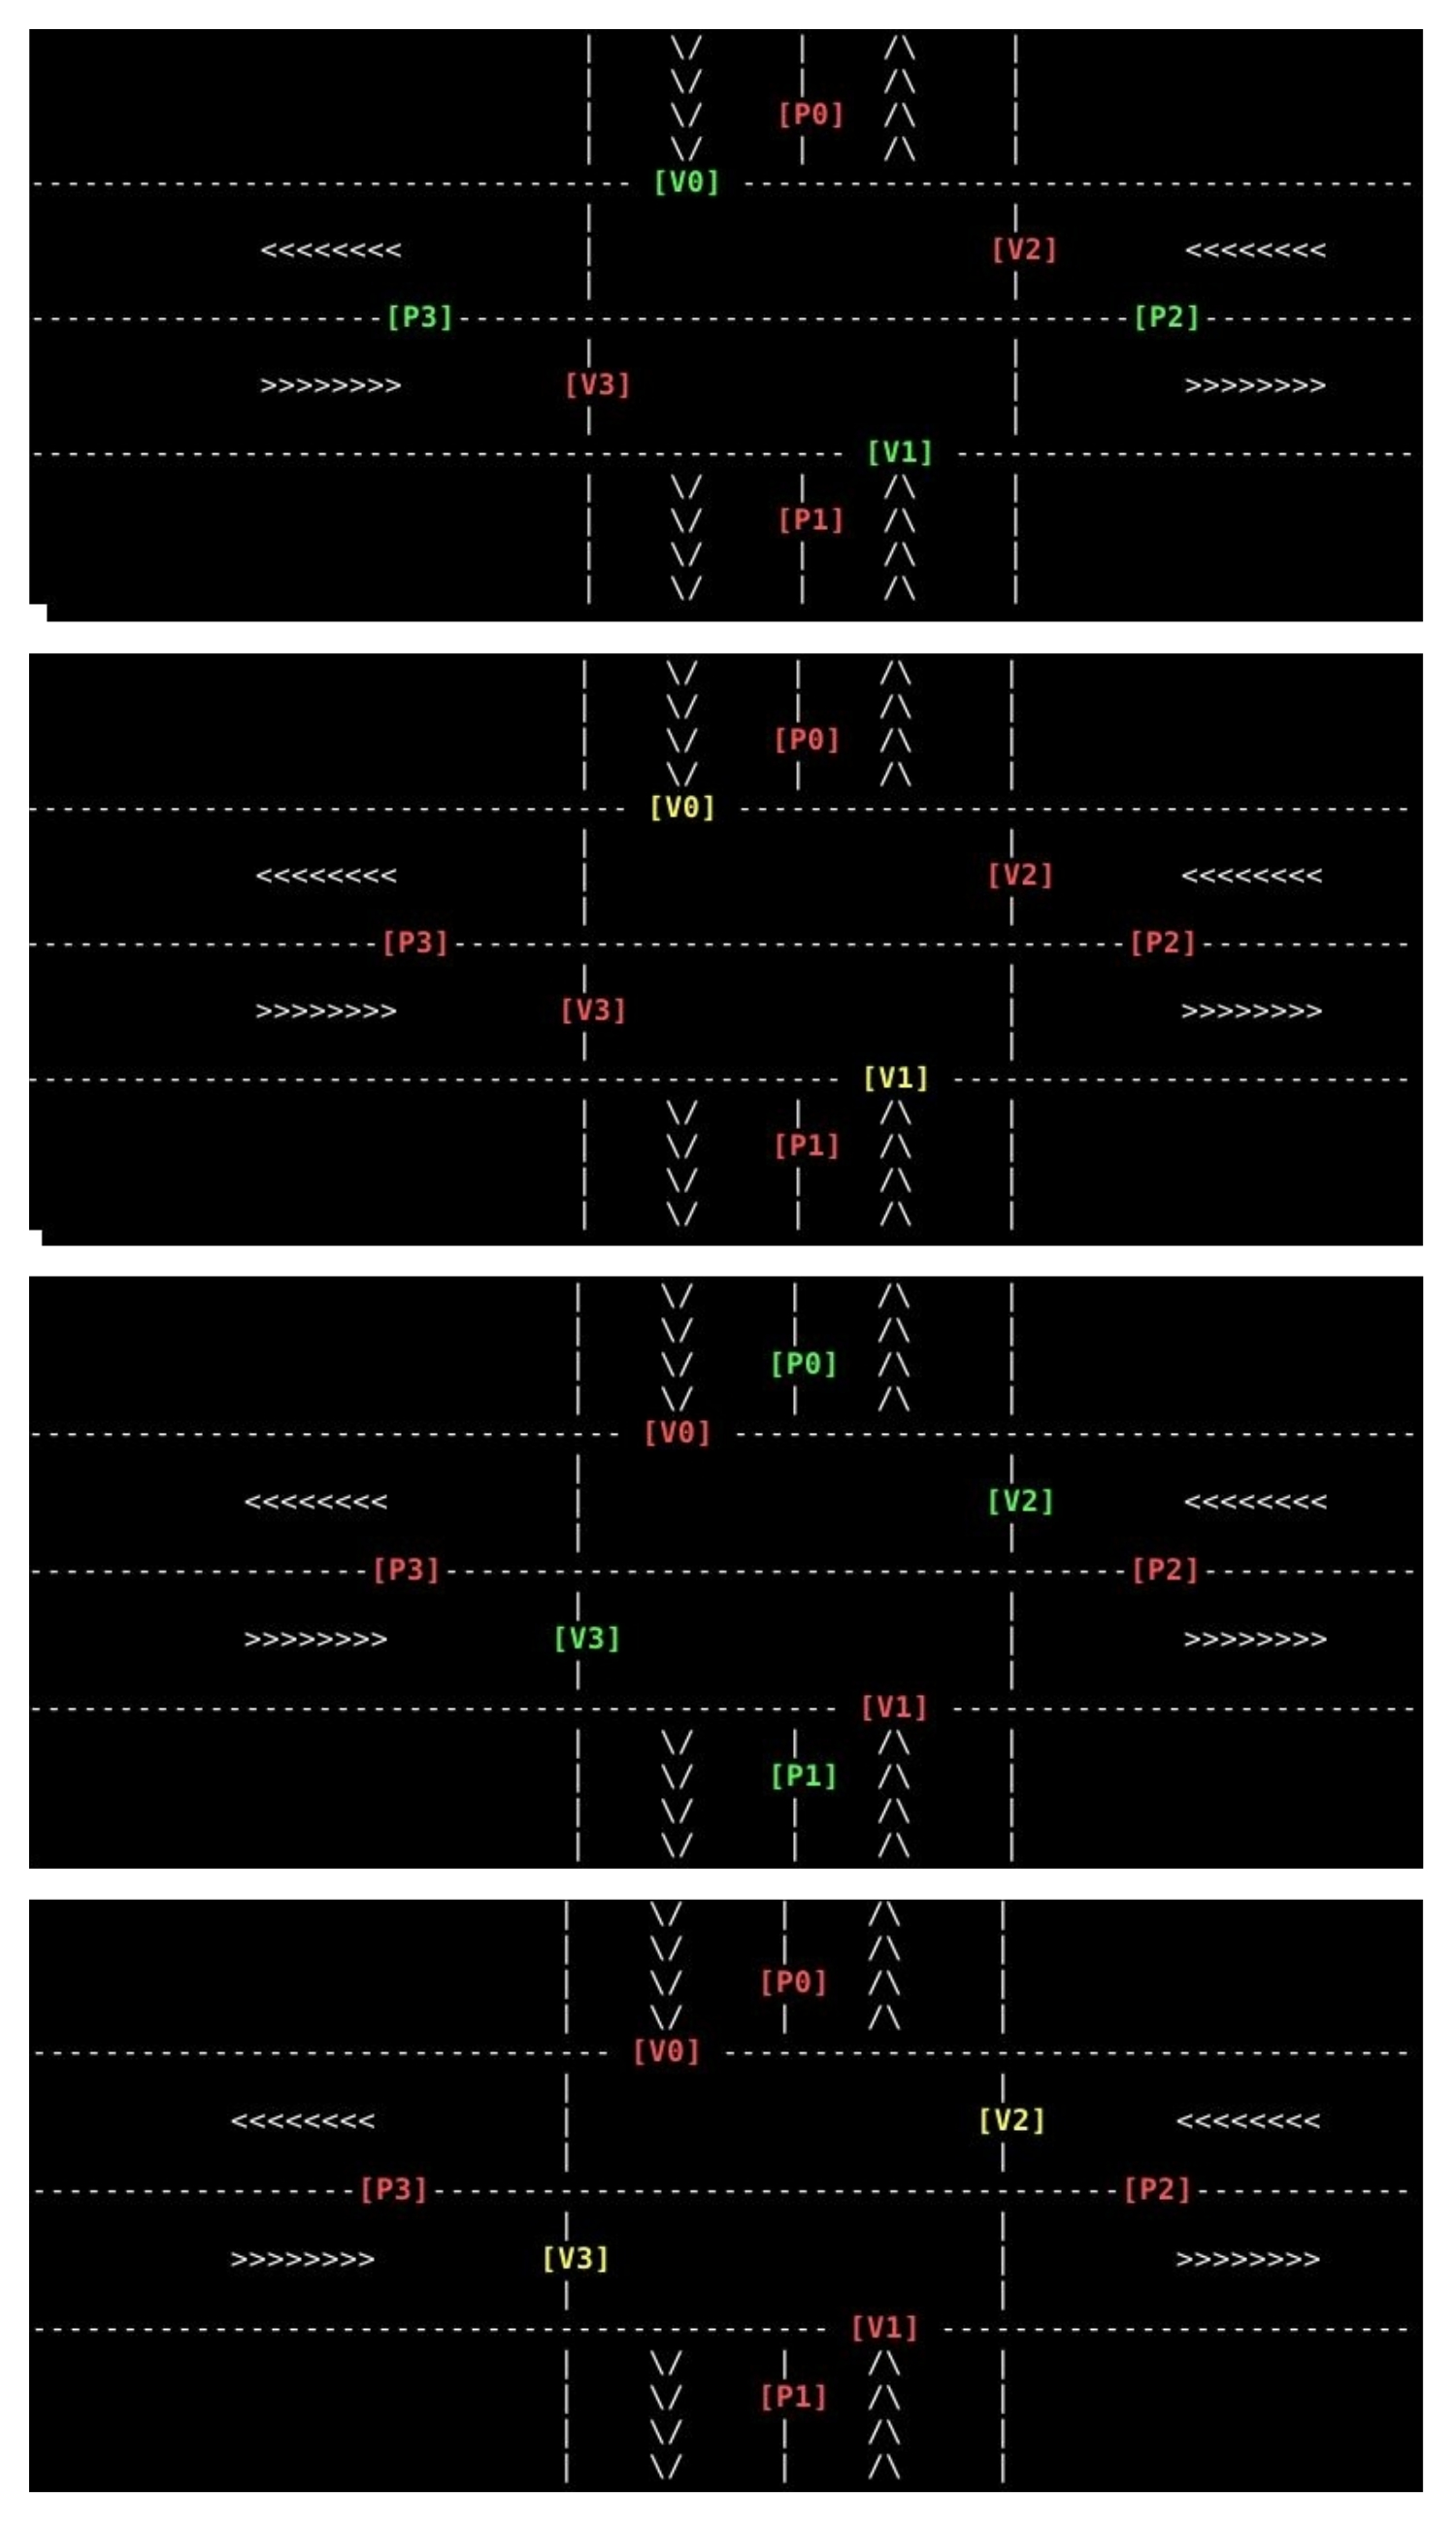
\includegraphics[width=12cm]{./images/Tasks.jpg}
\caption{Task-uri}
\label{fig:tasks}
\end{figure}
\newline\newline
Secven\c{t}e imposibile:

\begin{itemize}
\item Semafoarele de pe \c{s}oseaua vertical\u{a} \c{s}i cele de pe \c{s}oseaua orizontal\u{a} vor indica culoarea verde sau galben\u{a} \^{i}n acela\c{s}i timp;
\item Semafoarele pentru pietoni de pe o \c{s}osea sunt verzi \^{i}n timp ce semafoarele pentru vehicule de pe acea \c{s}osea sunt verzi sau galbene.
\end{itemize}

\section{Definirea structurii aplica\c{t}iei}

\subsection{Exemplu: Pas 3. Definirea taskurilor care compun aplica\c{t}ia}

\^{I}n cazul problemei noastre, acestea sunt taskurile:

\begin{itemize}
\item Task 1 (func\c{t}ia PerecheA) : \textbf{Task$\_$A}
\item Task 2 (func\c{t}ia Tranzi\c{t}ieAB) : \textbf{Task$\_$B}
\item Task 3 (func\c{t}ia PerecheB) : \textbf{Task$\_$C}
\item Task 4 (func\c{t}ia Tranzi\c{t}ieBA) : \textbf{Task$\_$D}
\end{itemize}

\section{Definirea solu\c{t}iei \^{i}n vederea implement\u{a}rii}

Am implementat solu\c{t}ia pentru problema aleas\u{a} \^{i}n \textit{Linux Xenomai / C}. Am creat c\^{a}te un fir de execu\c{t}ie pentru fiecare task \^{i}n parte, iar pentru a realiza comunicarea \^{i}ntre task-uri, am folosit semafoare binare. Deoarece intersec\c{t}ia trebuie s\u{a} \^{i}\c{s}i p\u{a}streze starea setat\u{a} de fiecare task pentru un anumit interval de timp, am folosit func\c{t}ia \textbf{\textit{sleep()}} \^{i}n cadrul firului de execu\c{t}ie corespunz\u{a}tor task-ului respectiv \^{i}nainte de a debloca task-ul urm\u{a}tor.

\subsection{Exemplu: Pas 4. Solu\c{t}ie de implementare}

Aleg mecanismele de sincronizare \c{s}i comunicare \^{i}ntre taskuri, prezent\^{a}nd organigramele taskurilor (vezi \autoref{fig:taskuri}):

\begin{itemize}
\item Am folosit 4 semafoare binare: SemPerecheA, SemPerecheB, SemTranzitieAB, SemTranzitieBA;
\item Am creat c\^{a}te un fir de execu\c{t}ie pentru fiecare task \^{i}n func\c{t}ia main, dup\u{a} care am folosit func\c{t}ia \textbf{\textit{sem$\_$post}} pentru a debloca task-ul 1 (PerecheA);
\item \^{I}n fiecare task, dup\u{a} setarea culorii corespunz\u{a}toare a semafoarelor, am folosit func\c{t}ia \textbf{\textit{Intersectie()}} pentru a reprezenta grafic culorile semafoarelor, dup\u{a} care am folosit func\c{t}ia \textbf{\textit{sleep()}} pentru a p\u{a}stra starea curent\u{a} a intersec\c{t}iei pentru un interval de timp stabilit \^{i}n prealabil;
\item La sf\^{a}r\c{s}itul acestui interval de timp este apelat\u{a} func\c{t}ia \textbf{\textit{sem$\_$post}} pentru a debloca semaforul task-ului urm\u{a}tor.
\end{itemize}

\begin{figure} [!htb]
\centering
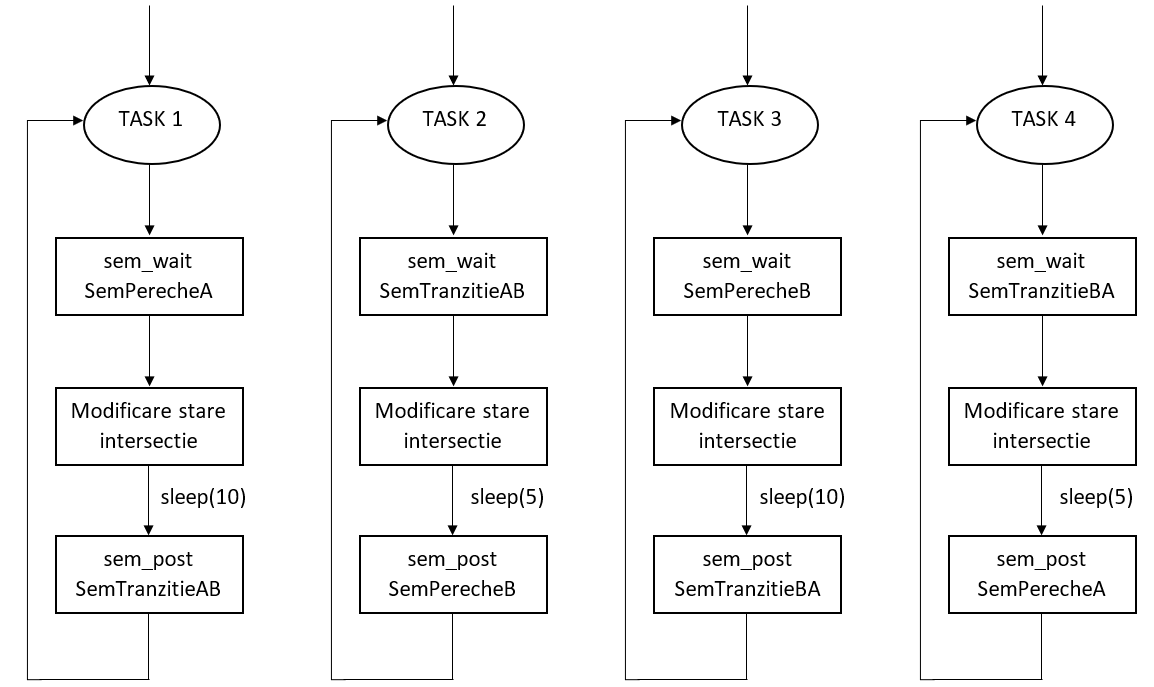
\includegraphics[width=12cm]{./images/SolutieImplementare.png}
\caption{\label{fig:taskuri}Solu\c{t}ie implementare - organigrame taskuri}
\end{figure} 


\section{Implementarea solu\c{t}iei}

\^{I}n aceast\u{a} sec\c{t}iune se va prezenta codul pentru implementare. 

\medskip
\medskip

\noindent
{\it \textbf{Linux Xenomai /C}:}
{\small
\begin{verbatim}
#include <stdlib.h>
#include <stdio.h>
#include <pthread.h>
#include <semaphore.h>
#include <stdbool.h>

#define RED "\e[1;31m"
#define GRN "\e[1;32m"
#define YEL "\e[1;33m"
#define ENDER "\033[0m"

struct semafor_vehicule{
	bool verde;
	bool galben;
	bool rosu;
};
typedef struct semafor_vehicule SEM_V;

struct semafor_pietoni{
	bool verde;
	bool rosu;
};
typedef struct semafor_pietoni SEM_P;

SEM_P P[4];
SEM_V V[4];
sem_t SemPerecheA, SemTranzitieAB, SemPerecheB, SemTranzitieBA;

void* PerecheA(void *);
void* TranzitieAB(void *);
void* PerecheB(void *);
void* TranzitieBA(void *);

void Intersectie(); // Ilustrare grafica a intersectiei (in culori)

void* (*functie[])(void*) = {PerecheA, TranzitieAB, PerecheB, TranzitieBA};

int main(void)
{
	pthread_t FIR[4];
	int i;
	
	sem_init(&SemPerecheA, 1, 0);
	sem_init(&SemTranzitieAB, 1, 0);
	sem_init(&SemPerecheB, 1, 0);
	sem_init(&SemTranzitieBA, 1, 0);
	
	for(i=0; i<4;i++)
		pthread_create(FIR+i,NULL,(void*)(*(functie+i)),NULL);
		
	sem_post(&SemPerecheA);
	
	for(i=0; i<4; i++)
		pthread_join(*(FIR+i), NULL);
		
	printf("Main: Toate firele de executie s-au terminat! \n");
	pthread_exit(NULL);
}

void* PerecheA(void *arg)
{
	int k;
	while(1)
	{
		sem_wait(&SemPerecheA);
		for(k = 0; k < 2; k++)
		{
			V[k].verde = true;
			V[k].rosu = false;
			V[k].galben = false;
			
			P[k].verde = false;
			P[k].rosu = true;
		}
		for(k = 2; k < 4; k++)
		{
			V[k].verde = false;
			V[k].rosu = true;
			V[k].galben = false;
			
			P[k].verde = true;
			P[k].rosu = false;
		}
		Intersectie();
		sleep(10);
		sem_post(&SemTranzitieAB);
	}
}

void* TranzitieAB(void *arg)
{
	int k;
	while(1)
	{
		sem_wait(&SemTranzitieAB);
		for(k = 0; k < 2; k++)
		{
			V[k].verde = false;
			V[k].rosu = false;
			V[k].galben = true;
			
			P[k].verde = false;
			P[k].rosu = true;
		}
		for(k = 2; k < 4; k++)
		{
			V[k].verde = false;
			V[k].rosu = true;
			V[k].galben = false;
			
			P[k].verde = false;
			P[k].rosu = true;
		}
		Intersectie();
		sleep(5);
		sem_post(&SemPerecheB);
	}
}

void* PerecheB(void *arg)
{
	int k;
	while(1)
	{
		sem_wait(&SemPerecheB);
		for(k = 0; k < 2; k++)
		{
			V[k].verde = false;
			V[k].rosu = true;
			V[k].galben = false;
			
			P[k].verde = true;
			P[k].rosu = false;
		}
		for(k = 2; k < 4; k++)
		{
			V[k].verde = true;
			V[k].rosu = false;
			V[k].galben = false;
			
			P[k].verde = false;
			P[k].rosu = true;
		}
		Intersectie();
		sleep(10);
		sem_post(&SemTranzitieBA);
	}
}

void* TranzitieBA(void *arg)
{
	int k;
	while(1)
	{
		sem_wait(&SemTranzitieBA);
		for(k = 0; k < 2; k++)
		{
			V[k].verde = false;
			V[k].rosu = true;
			V[k].galben = false;
			
			P[k].verde = false;
			P[k].rosu = true;
		}
		for(k = 2; k < 4; k++)
		{
			V[k].verde = false;
			V[k].rosu = false;
			V[k].galben = true;
			
			P[k].verde = false;
			P[k].rosu = true;
		}
		Intersectie();
		sleep(5);
		sem_post(&SemPerecheA);
	}
}

void Intersectie()
{
	system("clear");
    printf("	                       |    \\/     |    /\\     |\n");
    printf("	                       |    \\/     |    /\\     |\n");
    printf("	                       |    \\/    ");
 
    if(P[0].rosu) printf(RED);
	else if(P[0].verde) printf(GRN);
    printf("[P0]");
    printf(ENDER);
 
    printf("  /\\     |\n");
    printf("	                       |    \\/     |    /\\     |\n");
    printf("---------------------------------- ");
 
    if(V[0].rosu) printf(RED);
	else if(V[0].verde) printf(GRN);
	else if(V[0].galben) printf(YEL);
    printf("[V0]");
    printf(ENDER);
 
    printf(" -------------------------------------- \n");
    printf("                               |                       |\n");
    printf("             <<<<<<<<          |                      ");
 
    if(V[2].rosu) printf(RED);
	else if(V[2].verde) printf(GRN);
	else if(V[2].galben) printf(YEL);
    printf("[V2]");
    printf(ENDER);
 
    printf("       <<<<<<<<\n");
    printf("                               |                       |\n");
    printf("--------------------");
 
    if(P[3].rosu) printf(RED);
	else if(P[3].verde) printf(GRN);
    printf("[P3]");
    printf(ENDER);
 
    printf("--------------------------------------");
 
    if(P[2].rosu) printf(RED);
	else if(P[2].verde) printf(GRN);
    printf("[P2]");
    printf(ENDER);
 
    printf("------------ \n");
    printf("                               |                       |\n");
    printf("             >>>>>>>>         ");
 
    if(V[3].rosu) printf(RED);
	else if(V[3].verde) printf(GRN);
	else if(V[3].galben) printf(YEL);
    printf("[V3]");
    printf(ENDER);
 
    printf("                     |         >>>>>>>>\n");
    printf("                               |                       |\n");
    printf("---------------------------------------------- ");
 
    if(V[1].rosu) printf(RED);
	else if(V[1].verde) printf(GRN);
	else if(V[1].galben) printf(YEL);
    printf("[V1]");
    printf(ENDER);
 
    printf(" -------------------------- \n");
    printf("	                       |    \\/     |    /\\     |\n");
    printf("	                       |    \\/    ");
 
    if(P[1].rosu) printf(RED);
	else if(P[1].verde) printf(GRN);
    printf("[P1]");
    printf(ENDER);
 
    printf("  /\\     |\n");
    printf("	                       |    \\/     |    /\\     |\n");
    printf("	                       |    \\/     |    /\\     |\n");
}
\end{verbatim}
}


\section{Testarea aplica\c{t}iei si validarea solu\c{t}iei propuse}

\^{I}n final, am realizat ceea ce ne-am propus, rezultatele ob\c{t}inute fiind cele specificate \^{i}n cerin\c{t}\u{a}. \^{I}n urma execu\c{t}iei aplica\c{t}iei dezvoltate \^{i}n tem\u{a}, va rezulta reprezentarea grafic\u{a} din \autoref{fig:tasks}. 

\end{document}
